\documentclass[aspectratio=169]{beamer}
\usepackage{beamerthemesplit}
\usepackage{wrapfig}
\usetheme{SPbGU}
\usepackage{pdfpages}
\usepackage{array}
\usepackage{amsmath}
\usepackage{cmap} 
\usepackage[T2A]{fontenc} 
\usepackage[utf8]{inputenc}
\usepackage{indentfirst}
\usepackage{amsmath}
\usepackage{tikz}
\usepackage{multirow}
\usepackage[noend]{algpseudocode}
\usepackage{algorithm}
\usepackage{algorithmicx}
\usetikzlibrary{shapes,arrows}
\usepackage{fancyvrb}
\usepackage[english,russian]{babel}

\beamertemplatenavigationsymbolsempty


\title[UI]{Интерактивные пользовательские интерфейсы}
\subtitle[]{}
% То, что в квадратных скобках, отображается в левом нижнем углу. 
\institute[СПбГУ]{
Программная инженерия \\
Санкт-Петербургский государственный университет
}

\author[Кутуев Владимир]{Кутуев Владимир}
\date{3 апреля 2024г.}
\definecolor{orange}{RGB}{179,36,31}

\begin{document}
{
\begin{frame}
  
\includegraphics[width=1.7cm]{pictures/SPbGU_Logo.png}
  \vspace{-20pt}
  \begin{center}
    \titlepage
  \end{center}
\end{frame}
}

\begin{frame}[fragile]
  \transwipe[direction=90]
  \frametitle{Проблемы интерактивных приложений}
  
  \begin{itemize}
    \item Как заменить логику работы, не меняя интерфейс?
    \item Как заменить интерфейс, не меняя логику работы?
    \item Как реализовать логику и интерфейс на разных технологических стеках? (привет Web)
    \item Как сделать расширяемыми и логику и интерфейс?
  \end{itemize}

\end{frame}

\begin{frame}[fragile]
  \transwipe[direction=90]
  \frametitle{Одни данные разные представления}
  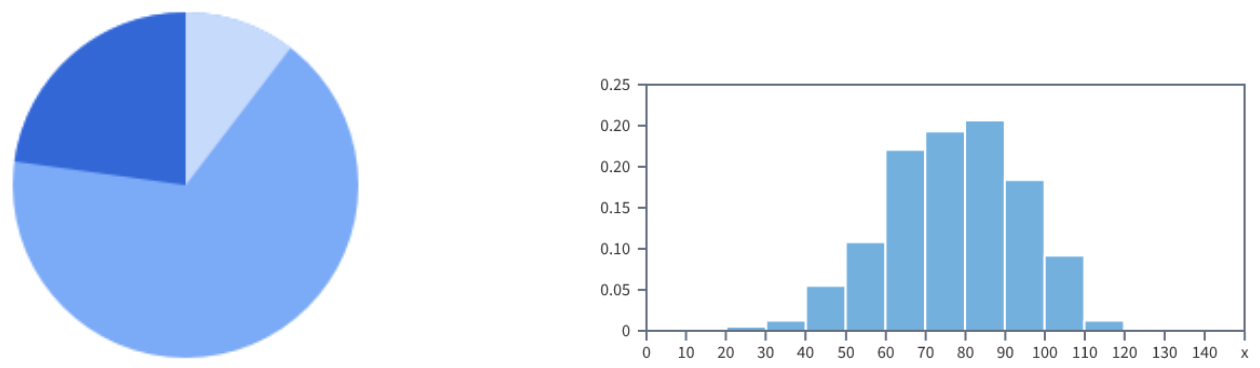
\includegraphics[width=.9\textwidth]{pictures/StatisticsView.png}

\end{frame}


\begin{frame}[fragile]
  \transwipe[direction=90]
  \frametitle{Задачи архитектуры приложений со сложным UI}
  
  \begin{itemize}
    \item Обработка действий пользователя
    \item Вызов основной логики/обновление данных
    \item Отображение изменений
    \item Объединить эти модули в единое приложение
  \end{itemize}

\end{frame}

\begin{frame}[fragile]
  \transwipe[direction=90]
  \frametitle{MV*-паттерны}
  \begin{itemize}
    \item Модель (Model) --- бизнес-логика
    \item Представление (View) --- пользовательский интерфейс
    \item * --- что-то
  \end{itemize}
  \begin{itemize}
    \item Model View Controller (MVC)
    \item Model View Presenter (MVP)
    \item Model View ViewModel (MVVM)
    \item Model View Adapter (MVA)
    \item Model View Intent (MVI)
  \end{itemize}

\end{frame}

\begin{frame}[fragile]
  \transwipe[direction=90]
  \frametitle{История MVС}
  \begin{minipage}{.65\textwidth}
    \begin{itemize}
      \item Трюгве Реенскауг (р. 1930)
      \item Исследовательский центр XEROX, 1978 год
      \item Первая реализация в языке - Smalltalk-80
      \item \href{https://folk.universitetetioslo.no/trygver/2003/javazone-jaoo/MVC_pattern.pdf}{\textcolor{blue}{Доклад автора про MVC}}
    \end{itemize}
  \end{minipage}
  \begin{minipage}{.31\textwidth}
      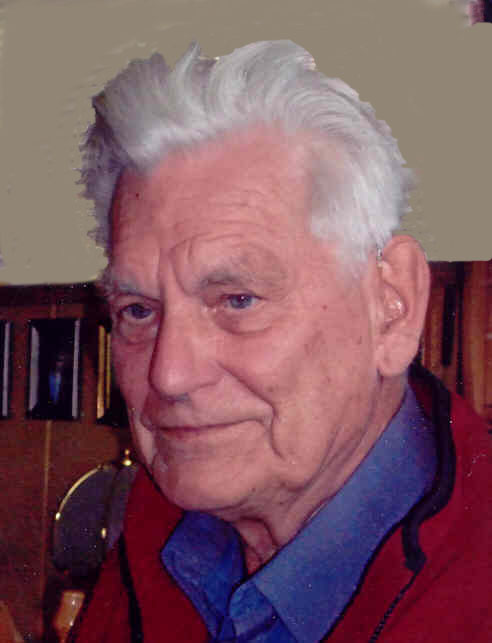
\includegraphics[width=5cm]{pictures/Trygve_Reenskaug.jpg}
  \end{minipage}

\end{frame}

\begin{frame}[fragile]
  \transwipe[direction=90]
  \frametitle{MVС}
  \begin{minipage}{.4\textwidth}
    \begin{itemize}
      \item Модель --- реализует бизнес-логику/хранит данные
      \item Контроллер --- обрабатывает запросы пользователя и вызывает обновление модели
      \item Представление --- отвечает за отображение данных пользователю
    \end{itemize}
  \end{minipage}
  \begin{minipage}{.56\textwidth}
    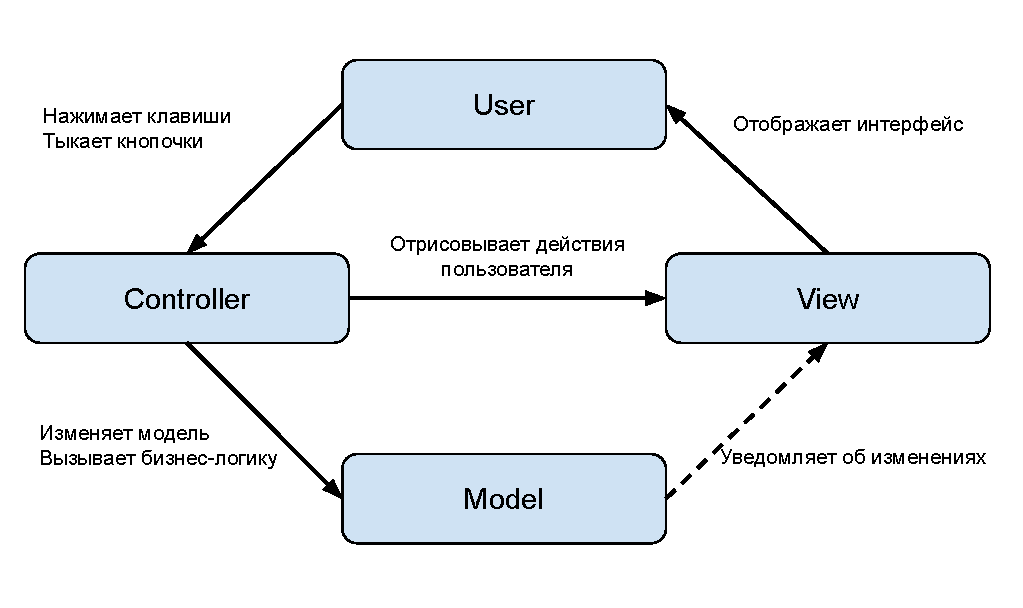
\includegraphics[width=9cm]{pictures/MVC.pdf}
  \end{minipage}

\end{frame}

\begin{frame}[fragile]
  \transwipe[direction=90]
  \frametitle{MVС-зоопарк}
  \begin{minipage}{.4\textwidth}
    \begin{itemize}
      \item Посмотрите на возможные \href{https://www.google.com/search?q=mvc}{\textcolor{blue}{варианты описания MVC}}
      \item В проектах ещё запутаннее
    \end{itemize}
  \end{minipage}
  \begin{minipage}{.56\textwidth}
    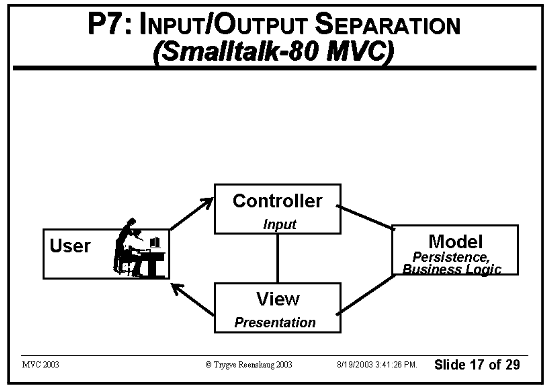
\includegraphics[width=9cm]{pictures/MVC_original.png}
  \end{minipage}

\end{frame}

\begin{frame}[fragile]
  \transwipe[direction=90]
  \frametitle{История MVP}
  \begin{itemize}
    \item Впервые появилась в IBM и более явно проявилась в системе Taligent  (1990-е)
    \item \href{http://www.wildcrest.com/Potel/Portfolio/mvp.pdf}{\textcolor{blue}{Одна из первых статей по MVP}}
  \end{itemize}
\end{frame}

\begin{frame}[fragile]
  \transwipe[direction=90]
  \frametitle{MVP}
  \begin{minipage}{.4\textwidth}
    \begin{itemize}
      \item Модель --- реализует бизнес-логику/хранит данные
      \item Представитель --- обрабатывает запросы от представления и вызывает обновление модели
      \item Представление --- обрабатывает запросы пользователя и отвечает за отображение данных пользователю
    \end{itemize}
  \end{minipage}
  \begin{minipage}{.56\textwidth}
    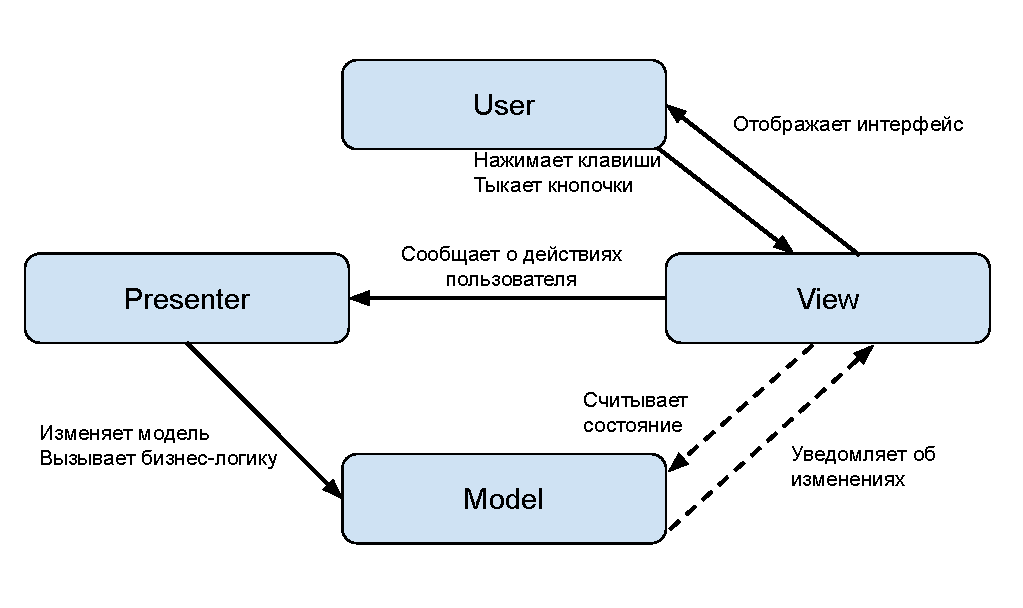
\includegraphics[width=9cm]{pictures/MVP.pdf}
  \end{minipage}
\end{frame}

\begin{frame}[fragile]
  \transwipe[direction=90]
  \frametitle{История MVVM}
  \begin{itemize}
    \item \href{https://learn.microsoft.com/en-us/archive/blogs/johngossman/introduction-to-modelviewviewmodel-pattern-for-building-wpf-apps}{\textcolor{blue}{Представлен Джоном Госсманом}} в 2005
    \item Развитие \href{https://martinfowler.com/eaaDev/PresentationModel.html}{\textcolor{blue}{шаблона Presentation Model}} Мартина Фаулера
  \end{itemize}
\end{frame}

\begin{frame}[fragile]
  \transwipe[direction=90]
  \frametitle{MVVM}
  \begin{minipage}{.4\textwidth}
    \begin{itemize}
      \item Модель --- реализует бизнес-логику/хранит данные
      \item Модель Представления --- хранит данные для представления, обрабатывает изменени пришедшие из модели и представления
      \item Представление --- обрабатывает запросы пользователя и отвечает за отображение данных пользователю
    \end{itemize}
  \end{minipage}
  \begin{minipage}{.56\textwidth}
    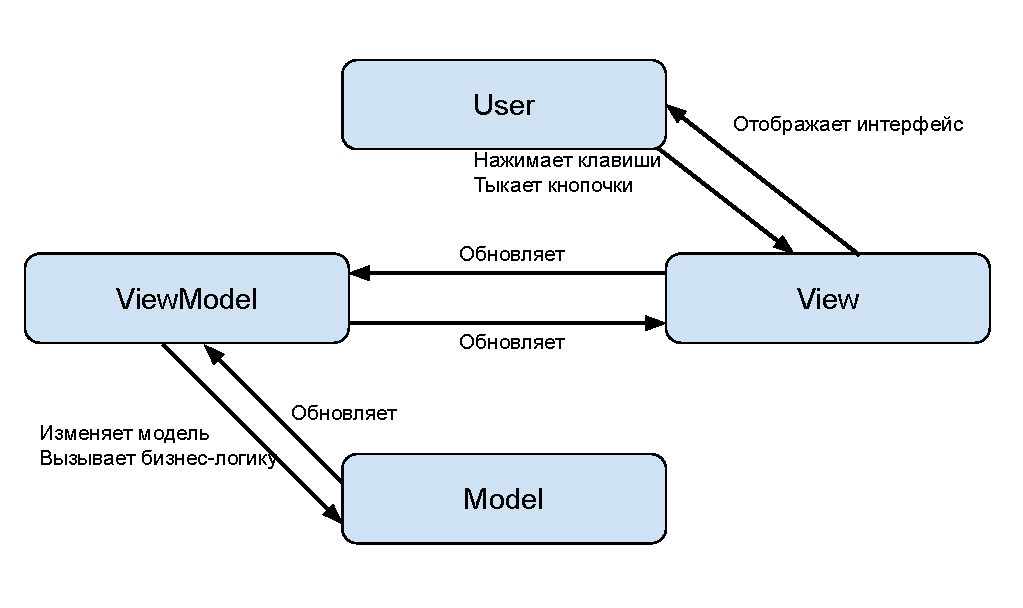
\includegraphics[width=9cm]{pictures/MVVM.pdf}
  \end{minipage}

\end{frame}


\end{document}
